\documentclass[letterpaper, 12pt]{article}
\usepackage[top=.5in,bottom=.5in,left=.75in,right=.75in,headheight=30pt, % as per the warning by fancyhdr
includehead,includefoot,
heightrounded, % to avoid spurious underfull messages
]{geometry}
\addtolength{\topmargin}{-.25in}
\usepackage{fancyhdr}
\usepackage{cancel}
\usepackage{gensymb}
\usepackage{xcolor}
\usepackage{tikz}
\usetikzlibrary{angles, quotes}
\usepackage{amssymb}
\pagestyle{fancy}
\usepackage{graphicx}
\usepackage{lastpage}
\usepackage{multicol}
\newcommand{\assnum}{Assignment 0.05}
\newcommand{\assname}{Dot and Cross Products}

\begin{document}
\fancyhead[l]{	\includegraphics[height=0.5in]{../Logo/sp.png} Name:}

\fancyfoot[c]{\thepage\ of \pageref{LastPage}}
\fancyfoot[r]{\assnum}	


\begin{center} \assnum{} - \assname{}
\end{center}





\begin{enumerate}
	\item Use the given vectors to calculate each of the following products:
	\begin{center}
			$\vec{A} = 2 \hat{i} + 6 \hat{j}$ \\
			$\vec{B} = 3 \hat{i} + 4 \hat{j}$
	\end{center}

	Find:
	\begin{enumerate}
		\item $\vec{A} \cdot \vec{B}$ 
		\vspace{0.5in}
		\item $\vec{A} \times \vec{B}$
		\vspace{0.5in}
		\item $\vec{B} \times \vec{A}$ 
		\vspace{0.5in}
	\end{enumerate}

	\item Use the given vectors to calculate each of the following products:
	\begin{center}
		$\vec{F} = 1 \hat{i} + 2 \hat{j} - 4 \hat{k} $ \\
		$\vec{G} = -5 \hat{i} - 3 \hat{j} + 2 \hat{k}$
	\end{center}
	
		Find:
	\begin{enumerate}
		\item $\vec{F} \cdot \vec{G}$ 
		\vspace{0.5in}
		\item $\vec{G} \cdot \vec{F}$
		\vspace{0.5in}
		\item $\vec{F} \times \vec{G}$ 
		\vspace{0.5in}
		\item $(\vec{F} \times \vec{G}) \cdot F$ 
		\vspace{0.5in}
	\end{enumerate}

\newpage
\item In the following diagram, $|\vec{C}| =  5m$ and $|\vec{D}| =  5.8 m$ 

\begin{center}
	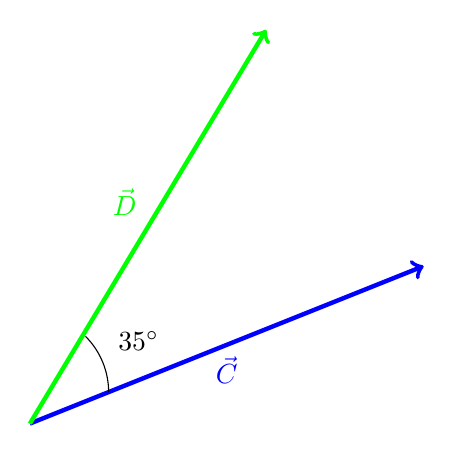
\begin{tikzpicture}
	\draw[->, ultra thick, blue](0,0) -- node[below] {$\vec{C}$} (5,2) ;
	\draw[->, ultra thick, green](0,0) -- node[anchor=south east] {$\vec{D}$} (3,5);
	
	\draw (1,.4) arc (0:45:1) ;
	\draw (1,1.3) -- (1,1.3) node[anchor=north west] {$35 \degree$};
	\end{tikzpicture}
\end{center}

Find:
\begin{enumerate}
	\item $\vec{C} \cdot \vec{D}$ 
	\vspace{0.5in}
	\item $|\vec{C} \times \vec{D}|$
	\vspace{0.5in}
	\end{enumerate}


\item Use the Right Hand Rule to determine the direction of the cross-product $\vec{L} \times \vec{M}$ in each of the following situations.  \textit{(Note: All answers will be ``Toward the left of the page," ``Toward the right of the page," ``Toward the top of the page," ``Toward the bottom of the page," ``Into the page," or ``out of the page.")}
\tikzset{
	pics/.cd,
	vector out/.style args={#1/#2}{
		code={
			\draw[#1] (0,0)  circle (.25);
			\draw[#2] (45:.25) -- (225:.25) (135:.25) -- (315:.25);
		}%end code   
	}%end style
}%end tikzset
\tikzset{
	pics/vector in/.style args={#1/#2/#3}{
		code={
			\draw[line width=#1] (0,0)  circle (.25);
			\fill[#2] (0,0)  circle (#3);
		}%end code   
	}%end style
}%end tikzset
\begin{center}
	\begin{tabular}{|c| c| c|}
		\hline 
	
			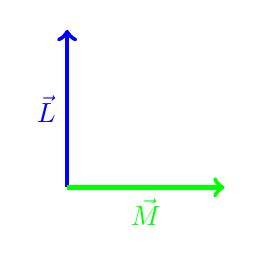
\begin{tikzpicture}
			\draw[->, ultra thick, blue](0,0) -- node[anchor=east] {$\vec{L}$} (0,2) ;
			\draw[->, ultra thick, green](0,0) -- node[anchor=north] {$\vec{M}$} (2,0);
			\end{tikzpicture}
	  & 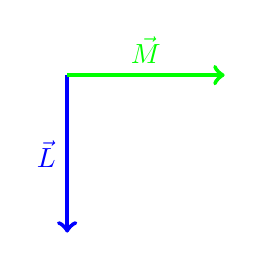
\begin{tikzpicture}
	  \draw[->, ultra thick, blue](0,0) -- node[anchor=east] {$\vec{L}$} (0,-2) ;
	  \draw[->, ultra thick, green](0,0) -- node[anchor=south] {$\vec{M}$} (2,0);
	  \end{tikzpicture}
	   & 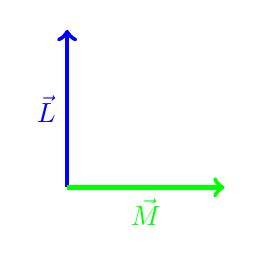
\begin{tikzpicture}
	   \draw[->, ultra thick, blue](0,0) -- node[anchor=east] {$\vec{L}$} (0,2) ;
	   \draw[->, ultra thick, green](0,0) -- node[anchor=north] {$\vec{M}$} (2,0);
	   \end{tikzpicture} \\
		\hline
		\begin{tikzpicture}%
		\draw[->, ultra thick, blue](0,0) -- node[anchor=east] {$\vec{L}$} (0,3) ;
		\path (0,0) pic {vector out={line width=1.5pt/line width=1.5pt}}   ;
		\draw[-, ultra thick](-.5,0) -- node[anchor=east] {$\vec{M}$} (-.5,0) ;
		
		\end{tikzpicture}
		
		 &
		 
		 		\begin{tikzpicture}%
		 \draw[->, ultra thick, blue](0,0) -- node[anchor=east] {$\vec{M}$} (0,3) ;
		 \draw[-, ultra thick](-.5,0) -- node[anchor=east] {$\vec{L}$} (-.5,0) ;
		 \path (0,0)  pic {vector in=1pt/blue/.1};
		 
		 \end{tikzpicture}
		 
		  & 
		  		\begin{tikzpicture}%
		  \draw[->, ultra thick, blue](0,0) -- node[anchor=south] {$\vec{L}$} (-3,0) ;
		  \path (0,0) pic {vector out={line width=1.5pt/line width=1.5pt}}   ;
		  \draw[-, ultra thick](.5,0) -- node[anchor=west] {$\vec{M}$} (.5,0) ;
		  
		  \end{tikzpicture}
		  
		  \\
		 \hline
		 
	\end{tabular}
\end{center}









 



\end{enumerate}
\end{document}
